\section{CAN bus transport layer implementation}

This section specifies the implementation of the CAN bus transport layer of UAVCAN.

Here and in the following parts of this section,
"CAN" implies both CAN 2.0 and CAN FD, unless specifically noted otherwise.
CAN FD should be considered the primary transport protocol.

UAVCAN utilizes only extended CAN frames with 29-bit identifiers.
UAVCAN can share the same bus with other protocols based on standard (non-extended) CAN frames with 11-bit identifiers.
However, future revisions of UAVCAN may utilize 11-bit identifiers as well;
therefore, backward compatibility with other protocols is not guaranteed.

\subsection{CAN ID structure}

UAVCAN utilizes three different CAN ID formats for different types of transfers:
message transfers, service transfers, and anonymous message transfers.
The structure is summarized on the figure \ref{fig:can_id_structure}.

% Please do not remove the hard placement specifier [H], it is needed to keep elements ordered.
\begin{figure}[H]
\centering
\setlength\arrayrulewidth{1pt}  % https://tex.stackexchange.com/a/256732/132781
\begin{tabu}{|c|X[c]|X[c]|X[c]|c|}
    \hline
    \rowfont{\bfseries}
    Bit & Service & Message & Anonymous message & Bit \\\hline

    28 & \multicolumn{3}{c|}{\multirow{3}{*}{Transfer priority}} & 28 \\
    27 & \multicolumn{3}{c|}{} & 27 \\
    26 & \multicolumn{3}{c|}{} & 26 \\
    \hline

    25 & \multicolumn{2}{c|}{Service not message} & \multirow{4}{*}{Reserved, required =0} & 25 \\\cline{2-3}
    24 & Request not response & \multirow{16}{*}{Message data type ID} & & 24 \\\cline{2-2}
    23 & \multirow{8}{*}{Service data type ID} & & & 23 \\
    22 & & & & 22 \\\cline{4-4}
    21 & & & \multirow{3}{*}{Message DTID modulo 8} & 21 \\
    20 & & & & 20 \\
    19 & & & & 19 \\\cline{4-4}
    18 & & & \multirow{10}{*}{Payload discriminator} & 18 \\
    17 & & & & 17 \\
    16 & & & & 16 \\\cline{2-2}
    15 & \multirow{7}{*}{Destination node ID} & & & 15 \\
    14 & & & & 14 \\
    13 & & & & 13 \\
    12 & & & & 12 \\
    11 & & & & 11 \\
    10 & & & & 10 \\
    9 & & & & 9 \\
    \hline

    8 & \multicolumn{3}{c|}{\multirow{7}{*}{Source node ID}} & 8 \\
    7 & \multicolumn{3}{c|}{} & 7 \\
    6 & \multicolumn{3}{c|}{} & 6 \\
    5 & \multicolumn{3}{c|}{} & 5 \\
    4 & \multicolumn{3}{c|}{} & 4 \\
    3 & \multicolumn{3}{c|}{} & 3 \\
    2 & \multicolumn{3}{c|}{} & 2 \\
    \hline

    1 & \multicolumn{3}{c|}{\multirow{2}{*}{Data type major version number modulo 4}} & 1 \\
    0 & \multicolumn{3}{c|}{} & 0 \\
    \hline
    \rowfont{\bfseries}
    Bit & Service & Message & Anonymous message & Bit \\\hline
\end{tabu}
\caption{CAN ID structure}\label{fig:can_id_structure}
\end{figure}

The fields are described in detail in the following sections.
The tables \ref{table:can_id_fields_message_transfer},
\ref{table:can_id_fields_anonymous_message_transfer}, and \ref{table:can_id_fields_service_transfer}
summarize the purpose of the fields and their permitted values
for message transfers, anonymous message transfers, and service transfers, respectively.
The following acronyms are used for brevity:
\begin{description}
    \item[DTID] - data type ID.
    \item[DTMVN] - data type major version number.
\end{description}

\begin{UAVCANSimpleTable}{CAN ID fields for message transfers}{|l l l X|}
    \label{table:can_id_fields_message_transfer}
    Field               & Width & Permitted values  & Description \\
    Transfer priority   & 3     & [0, 7] (any)      & Section \ref{sec:transfer_prioritization}. \\
    Service not message & 1     & 0                 & Always zero for message transfers. \\
    Message DTID        & 16    & [0, 65535] (any)  & Data type ID of the encoded message data structure. \\
    Source node ID      & 7     & [1, 127]          & Node ID of the origin. \\
    Message DTMVN       & 2     & [0, 3] (any)      & Major version number of the data type, modulo 4. \\
\end{UAVCANSimpleTable}

\begin{UAVCANSimpleTable}{CAN ID fields for anonymous message transfers}{|l l l X|}
    \label{table:can_id_fields_anonymous_message_transfer}
    Field               & Width & Permitted values  & Description \\
    Transfer priority   & 3     & [0, 7] (any)      & Section \ref{sec:transfer_prioritization}. \\
    Reserved field      & 4     & 0                 & Set to zero when emitting. When receiving, ignore the
                                                      frame if this field is not zero. \\
    Message DTID modulo 8& 3    & [0, 7] (any)      & Three least significant bits of the data type ID of the
                                                      encoded message data structure. Message types where DTID is
                                                      greater than 7 cannot be used with anonymous message transfers. \\
    Payload discriminator & 10  & [0, 1023] (any)   & Used for CAN ID conflict avoidance;
                                                      see section \ref{sec:can_payload_discriminator}. \\
    Source node ID      & 7     & 0                 & Set to zero. This field is used to distinguish anonymous message
                                                      transfers from regular message transfers. \\
    Message DTMVN       & 2     & [0, 3] (any)      & Major version number of the data type, modulo 4. \\
\end{UAVCANSimpleTable}

\begin{UAVCANSimpleTable}{CAN ID fields for service transfers}{|l l l X|}
    \label{table:can_id_fields_service_transfer}
    Field               & Width & Permitted values  & Description \\
    Transfer priority   & 3     & [0, 7] (any)      & Section \ref{sec:transfer_prioritization}. \\
    Service not message & 1     & 1                 & Always one for service transfers. \\
    Request not response& 1     & \{0, 1\} (any)    & 1 for service request, 0 for service response. \\
    Service DTID        & 8     & [0, 255] (any)    & Data type ID of the encoded service data structure
                                                      (request or response). \\
    Destination node ID & 7     & [1, 127]          & Node ID of the destination
                                                      (i.e., server for requests, client for responses). \\
    Source node ID      & 7     & [1, 127]          & Node ID of the origin
                                                      (i.e., client for requests, server for responses). \\
    Service DTMVN       & 2     & [0, 3] (any)      & Major version number of the data type, modulo 4. \\
\end{UAVCANSimpleTable}

\subsubsection{Transfer priority}

Valid values for priority range from 0 to 7, inclusively,
where 0 corresponds to the highest priority, and 7 corresponds to the lowest priority.
Mnemonics for transfer priority levels are provided in the section \ref{sec:transfer_prioritization}.

In multi-frame transfers, the value of the priority field must be identical for all frames of the transfer.

Shall there be multiple transfers of different types at the same priority level contesting for the bus access,
the following precedence is ensured, from higher priority to lower priority:

\begin{enumerate}
    \item Message transfers.
    \item Service response transfers.
    \item Service request transfers.
\end{enumerate}

Message transfers take precedence over service transfers because message broadcasting is the primary method of
communication in UAVCAN networks.
Service responses take precedence over service requests in order to make service invocations more atomic
and reduce the number of pending states in the system.

Within the same type and the same priority level,
transfers are prioritized according to the data type ID:
transfers with lower data type ID values preempt those with higher data type ID values.

\subsubsection{Data type ID}

A higher-level review of the concept of data type ID is available in the chapter \ref{sec:dsdl}.

For anonymous message transfers, the range of usable message type ID values is limited to [0,~7];
messages with data type ID outside of this range cannot be used with anonymous message
transfers with this transport.

\subsubsection{Data type major version number}

As explained in the section \ref{sec:dsdl_versioning},
the difference between the lowest and the highest released major version numbers of any given data type
may never exceed three.

Having made certain assumptions about the data type release cadence and the deprecation strategy,
one can see that the transport layer can represent the data type major version number using a reduced
modulo 4 representation; i.e., instead of carrying the whole version number, the transport layer
can carry only the major version number modulo four:
$$V^\prime{} = V \bmod 4 \Leftrightarrow{} V \geq{} 0$$
where $V$ is the data type major version number and $V^\prime{}$ is its reduced representation used by
the transport layer.

Taking advantage of the fact that the transport layer representation of the major data type version number
belongs to [0, 3], UAVCAN uses only a two-bit wide field in the CAN identifier to represent the major
version number.

The bit width saving measures described here warrant certain special handling rules for the major version
number at the transport layer.
When emitting a transfer, the node must compute the modulo of the major data type version number
as described above, and populate the corresponding CAN ID field with the resulting value.
When receiving a transfer, the node must search for an appropriate data type definition
among the known definitions by looking for the one which has the same major version number modulus
as the received modulus:
$$V_\text{local} \bmod 4 = V^\prime{}$$
where $V_\text{local}$ is the major version number of the locally available data type definition that will be used
to process the transfer.

From the above description one can see that a data type mismatch will occur if the absolute difference between
the major data type version used by the emitter and that used by the receiver exceeds three:
$$V_\text{local} \neq V \Leftrightarrow{} \vert{}V_\text{local} - V\vert{} \geq 4$$
However, due to the implicit deprecation policy defined in the section \ref{sec:dsdl_versioning},
the risk of version conflict is easy to avoid, and the limitation is therefore deemed acceptable.

\subsubsection{Node ID}

Valid values of node ID belong to the range [1, 127].

Node ID is represented by a 7-bit unsigned integer value; zero is reserved.
A node ID of zero is used to represent either an unknown node or all nodes, depending on the context.

As such, for anonymous message transfers, the source node ID field is always set to zero.
By observing a source node ID of zero, receiving nodes can distinguish
anonymous message transfers from other types of transfers.

\subsubsection{Payload discriminator}\label{sec:can_payload_discriminator}

CAN bus does not allow different nodes to transmit CAN frames with different data field values under the same CAN ID.
Owing to the fact that the CAN ID includes the node ID value of the transmitting node,
this restriction does not affect regular UAVCAN transfers.
However, anonymous message transfers would violate this restriction,
because they all share the same node ID of zero.

In order to work-around this problem,
UAVCAN adds a \emph{payload discriminator} to the CAN ID of anonymous message transfers,
and defines special logic for handling CAN bus errors during transmission of anonymous frames.

The payload discriminator field must be filled with pseudorandom data whenever a node transmits an
anonymous message transfer.
The source of the pseudorandom data must be likely to produce different discriminator values
for different data field values.
A possible way of initializing the payload discriminator value is to apply the transfer CRC function
(as defined in the section \ref{sec:transfer_crc})
to the contents of the anonymous message, and then use any 10 bits of the result.
Nodes that adopt this approach will be using the same payload discriminator value for identical messages,
which is acceptable since this will not trigger an error on the bus.

Since the discriminator is only 10 bits long,
the probability of having multiple nodes emitting CAN frames with the same CAN ID
but different data can exceed 0.1\%, which is significant.
Therefore, the protocol must account for possible errors on the CAN bus triggered by CAN ID collisions.
In order to comply with this requirement,
UAVCAN requires all nodes to immediately abort transmission of all anonymous transfers once an error on
the CAN bus is detected.
This measure allows the protocol to prevent the bus deadlock that may occur if the automatic
retransmission on bus error is not suppressed.

\subsection{CAN frame data}

The CAN frame data field may contain the following data items, in the listed order:
\begin{enumerate}
    \item The useful payload (serialized data structure). This segment may be empty.
    \item Possible padding bytes.
          Padding bytes may be necessary if the transport layer does not provide byte-level
          granularity of the data field length (e.g., CAN FD).
    \item The last frame of multi-frame transfers always contains the transfer CRC (section \ref{sec:transfer_crc}).
    \item The last byte of the data field always contains the \emph{tail byte}.
\end{enumerate}
The segments are documented below in this section.

\subsubsection{Tail byte}

UAVCAN adds one byte of overhead to every CAN frame irrespective of the type of the transfer.
The extra byte contains certain metadata for the needs of the transport layer.
It is named the \emph{tail byte}, and as the name suggests, it is always situated
at the very last byte of the data field of every CAN frame.
The tail byte contains four fields: \emph{start of transfer}, \emph{end of transfer},
\emph{toggle bit}, and the transfer ID (described earlier in the section \ref{sec:transfer_id}).
The placement of the fields and their usage for single-frame and multi-frame transfers
are documented in the table \ref{table:can_tail_byte}.

% Please do not remove the hard placement specifier [H], it is needed to keep tables ordered.
\begin{table}[H]\caption{Tail byte structure}\label{table:can_tail_byte}
\begin{tabu}{|c|l|X[2]|X[3]|}
    \hline
    \rowfont{\bfseries}
    Bit & Field & Single-frame transfers & Multi-frame transfers \\
    \hline

    7   & Start of transfer & Always 1  & First frame: 1, otherwise 0. \\\hline
    6   & End of transfer   & Always 1  & Last frame: 1, otherwise 0. \\\hline
    5   & Toggle bit        & Always 1  & First frame: 1, then alternates; section \ref{sec:toggle_bit}. \\\hline

    4   &               & \multicolumn{2}{c|}{} \\
    3   &               & \multicolumn{2}{c|}{Modulo 32 (range [0, 31])} \\
    2   & Transfer ID   & \multicolumn{2}{c|}{section \ref{sec:transfer_id}} \\
    1   &               & \multicolumn{2}{c|}{} \\
    0   &               & \multicolumn{2}{c|}{\footnotesize{(least significant bit)}} \\
    \hline
\end{tabu}
\end{table}

The transfer ID field is populated according to the specification provided in the section \ref{sec:transfer_id}.
The usage of this field is independent of the type of the transfer.

For single-frame transfers, the fields start-of-transfer, end-of-transfer, and the toggle bit
are all set to~1.

For multi-frame transfers, the fields start-of-transfer and end-of-transfer
are used to state the boundaries of the current transfer as described in the table.
The transfer ID value is identical for all frames of a multi-frame transfer.

The toggle bit, as described in the section \ref{sec:toggle_bit}, serves
two main purposes: CAN frame deduplication and protocol version detection.

\subsubsection{Padding bytes}

Certain transports (such as CAN FD) may not provide byte-level granularity of the CAN data field length.
In that case, the useful payload is to be padded with the minimal number of padding bytes required
to bring the total length of the CAN data field to a value that can satisfy the length granularity constraints.

When transmitting, each padding byte must be set to $\text{85} = \text{55}_\text{hex} = \text{0101\,0101}_\text{bin}$.
This specific padding value is chosen to avoid stuff bits and to facilitate CAN controller synchronization.

When receiving, the values of the padding bytes must be ignored.
In other words, receiving nodes must not make any assumptions about the values of the
padding bytes.

Usage of padding bytes implies that when a serialized message is being deserialized by a receiving node,
the byte sequence used for deserialization may be longer than the actual byte sequence generated by the
emitting node during serialization.
Therefore, nodes must ignore the trailing unused data bytes at the end of serialized byte sequences;
a length mismatch is only to be considered an error if the received byte sequence is shorter
than expected by the deserialization routine.

\subsubsection{Single-frame transfers}

For single-frame transfers, the data field of the CAN frame contains two or three segments:
the useful payload (which is the serialized data structure, may be empty), possible padding bytes,
and the tail byte (the last byte of the data field).

The resulting data field segmentation is shown in the table \ref{table:can_data_segments_single_frame}.

\begin{table}[H]\caption{CAN frame data segments for single-frame transfers}
\label{table:can_data_segments_single_frame}
\begin{tabu}{|l l X|}
    \hline
    \rowfont{\bfseries}
    Offset                  & Length                     & Segment \\\hline
    $0$                     & $L_\text{payload}\geq{}0$  & Useful payload (serialized data structure). \\\hline
    $L_\text{payload}$      & $L_\text{padding}\geq{}0$  & Padding bytes (if necessary). \\\hline
    $L_\text{payload} + L_\text{padding}$ & $1$          & Tail byte. \\\hline
\end{tabu}
\end{table}

\subsubsection{Multi-frame transfers}

For multi-frame transfers, all frames except the last one contain only a fragment
of the useful payload and the tail byte.
Notice that the padding bytes are not used in multi-frame transfers, excepting the last frame.

The useful payload is fragmented in the forward order: the first CAN frame of a multi-frame transfer
contains the beginning of the payload (the first fragment),
the following frames contain the subsequent fragments of the useful payload.
The last CAN frame of a multi-frame transfer contains the last fragment, unless
the last fragment was fully accommodated by the previous CAN frame of the transfer.
In the latter case, the last CAN frame will contain only the metadata,
as specified below in this section.

Each CAN frame of a multi-frame transfer except the last one
should use the maximum CAN data length permitted by the transport.
Observe that this is not a hard requirement;
some systems that utilize CAN FD may opt for shorter CAN frames in order to reduce the worst case
preemption latency.
Therefore, UAVCAN implementations must be able to correctly process multi-frame transfers with arbitrary
CAN frame data lengths.

The resulting data field segmentation for all frames of a multi-frame transfer except the last one is
shown in the table \ref{table:can_data_segments_multi_frame_not_last}.

\begin{table}[H]\caption{CAN frame data segments for multi-frame transfers (except the last CAN frame of the transfer)}
\label{table:can_data_segments_multi_frame_not_last}
\begin{tabu}{|l l X|}
    \hline
    \rowfont{\bfseries}
    Offset                  & Length                & Segment \\\hline
    $0$                     & $L_\text{payload}>0$  & A fragment of the useful payload (serialized data structure).
                                                      This segment occupies the entirety of the CAN data field
                                                      except the last byte, which is used by the tail byte. \\\hline
    $L_\text{payload}$      & $1$                   & Tail byte. \\\hline
\end{tabu}
\end{table}

The last CAN frame of a multi-frame transfer contains one or two additional segments:
the padding bytes (if necessary) and the transfer CRC.
The padding rules are identical to those of single-frame transfers.
The transfer CRC is to be allocated in the big-endian byte order\footnote{Most significant byte first.
This byte order is used to allow faster CRC residue checks; more info in section \ref{sec:transfer_crc}.}
immediately before the tail byte.
The resulting data field segmentation is shown in the table \ref{table:can_data_segments_multi_frame_last}.

\begin{table}[H]\caption{CAN frame data segments for multi-frame transfers (the last CAN frame of the transfer)}
\label{table:can_data_segments_multi_frame_last}
\begin{tabu}{|l l X|}
    \hline
    \rowfont{\bfseries}
    Offset                  & Length                     & Segment \\\hline
    $0$                     & $L_\text{payload}\geq{}0$  & The last fragment of the useful payload
                                                           (serialized data structure). \\\hline
    $L_\text{payload}$      & $L_\text{padding}\geq{}0$  & Padding bytes (if necessary). \\\hline

    \multirow{2}{*}{$L_\text{payload} + L_\text{padding}$} & \multirow{2}{*}{$2$} &
                                                           Transfer CRC, high byte.\\
                            &                            & Transfer CRC, low byte.\\\hline

    $L_\text{payload} + L_\text{padding} + 2$ & $1$        & Tail byte. \\\hline
\end{tabu}
\end{table}

\subsection{CAN-related software design considerations}

\subsubsection{Ordered transmission}

Multi-frame transfers use identical CAN ID for all frames of the transfer,
and UAVCAN requires that all frames of a multi-frame transfer should be transmitted in the correct order.
Therefore, the CAN controller driver software must ensure that CAN frames with identical CAN ID values
must be transmitted in their order of appearance in the transmission queue.
Some CAN controllers will not meet this requirement by default,
so the designer must take special care to ensure the correct behavior, and apply workarounds if necessary.

\subsubsection{Transmission time-stamping}

Certain advanced features of UAVCAN may require the driver to time-stamp outgoing transport frames, e.g.,
the time synchronization feature.
A sensible approach to transmission time-stamping is built around the concept of \emph{loop-back frames},
which is described here.

If the application needs to time-stamp an outgoing frame, it sets a special flag -- the \emph{loop-back flag} --
on the frame before sending it to the driver.
The driver would then automatically re-enqueue this frame back into the reception queue once it is transmitted
(keeping the loop-back flag set so that the application is able to distinguish the loop-back
frame from regular received traffic).
The time-stamp of the loop-backed frame would be of the moment when it was delivered to the bus.

The advantage of the loop-back based approach is that it relies on the same interface between
the application and the driver that is used for regular communications.
No complex and dangerous callbacks or write-backs from interrupt handlers are involved.

\subsubsection{Inner priority inversion}

Suppose the application needs to emit a frame with the CAN ID $X$.
The frame is submitted to the CAN controller's registers and the transmission is started.
Suppose that afterwards it turned out that there is a new frame with the CAN ID $(X-1)$ that needs to be sent,
too, but the previous frame $X$ is in the way, and it is blocking the transmission of the new frame.
This may turn into a problem if the lower-priority frame is losing arbitration on the bus due
to the traffic on the bus having higher priority than the current frame,
but lower priority than the next frame that is waiting in the queue.

A naive solution to this is to continuously check whether the priority of the frame that is currently being
transmitted by the CAN controller is lower than the priority of the next frame in the queue, and if it is,
abort transmission of the current frame, move it back to the transmission queue,
and begin transmission of the new one instead.
This approach, however, has a hidden race condition:
the old frame may be aborted at the moment when it has already been received by remote nodes,
which means that the next time it is re-transmitted, the remote nodes will see it duplicated.
Additionally, this approach increases the complexity of the driver and can possibly affect
its throughput and latency.

Most CAN controllers offer a proper solution to the problem:
they have multiple transmission mailboxes (usually at least 3),
and the controller always chooses for transmission the mailbox which contains the highest priority frame.
This provides the application with a possibility to avoid the inner priority inversion problem:
whenever a new transmission is initiated, the application should check whether the priority of the next frame
is higher than any of the other frames that are already awaiting transmission.
If there is at least one higher-priority frame pending,
the application doesn't move the new one to the controller's transmission mailboxes,
it remains in the queue.
Otherwise, if the new frame has a higher priority level than all of the pending frames,
it is pushed to the controller's transmission mailboxes and removed from the queue.
In the latter case, if a lower-priority frame loses arbitration,
the controller would postpone its transmission and try transmitting the higher-priority one instead.
That resolves the problem.

There is an interesting extreme case, however.
Imagine a controller equipped with $N$ transmission mailboxes.
Suppose the application needs to emit $N$ frames in the increasing order of priority,
which leads to all of the transmission mailboxes of the controller being occupied.
Now, if all of the conditions below are satisfied, the system ends up with a priority inversion condition nevertheless,
despite the measures described above:

\begin{itemize}
    \item The highest-priority pending CAN frame cannot be transmitted due to the bus being saturated
    with a higher-priority traffic.
    \item The application needs to emit a new frame which has a higher priority than that which saturates the bus.
\end{itemize}

If both hold, a priority inversion is afoot because there is no free transmission mailbox to
inject the new higher-priority frame into.
The scenario is extremely unlikely, however;
it is also possible to construct the application in a way that would preclude the problem,
e.g., by limiting the number of simultaneously used distinct CAN ID values.

The following pseudocode demonstrates the principles explained above:

\begin{minipage}{0.8\textwidth}
\begin{minted}{cpp}
// Returns the index of the TX mailbox that can be used for the transmission of the newFrame
// If none are available, returns -1.
getFreeMailboxIndex(newFrame)
{
    chosen_mailbox = -1     // By default, assume that no mailboxes are available

    for i = 0...NumberOfTxMailboxes
    {
        if isTxMailboxFree(i)
        {
            chosen_mailbox = i
            // Note: cannot break here, must check all other mailboxes as well.
        }
        else
        {
            if not isFramePriorityHigher(newFrame, getFrameFromTxMailbox(i))
            {
                chosen_mailbox = -1
                break   // Denied - must wait until this mailbox has finished transmitting
            }
        }
    }

    return chosen_mailbox
}
\end{minted}
\end{minipage}

\subsubsection{Automatic hardware acceptance filter configuration}

Most CAN controllers are equipped with hardware acceptance filters.
Hardware acceptance filters reduce the application workload by ignoring irrelevant CAN frames on the bus
by comparing their ID values against the set of relevant ID values configured by the application.

There exist two common approaches to CAN hardware filtering:
list-based and mask-based.
In the case of the list-based approach, every CAN frame detected on the bus is compared
against the set of reference CAN ID values provided by the application;
only those frames that are found in the reference set are accepted.
Due to the complex structure of the CAN ID field used by UAVCAN,
usage of the list-based filtering method with this protocol is impractical.

Most CAN controller vendors implement mask-based filters,
where the behavior of each filter is defined by two parameters: the mask $M$ and the reference ID $R$.
Then, such filter accepts only those CAN frames for which the following bitwise logical condition holds
true\footnote{$\land$ -- bitwise logical AND, $\oplus$ -- bitwise logical XOR, $\neg$ - bitwise logical NOT.}:
$$((X \land M) \oplus R) \leftrightarrow 0$$
where $X$ is the CAN ID value of the evaluated frame.

Complex UAVCAN applications are often required to operate with more distinct transfers than there are
acceptance filters available in the hardware.
That creates the challenge of finding the optimal configuration of the available filters that meets the
following criteria:
\begin{itemize}
    \item All CAN frames needed by the application are accepted.
    \item The number of irrelevant frames (i.e., not used by the application) accepted from the bus is minimized.
\end{itemize}

The optimal configuration is a function of the number of available hardware filters,
the set of distinct transfers needed by the application,
and the expected frequency of occurrence of all possible distinct transfers on the bus.
The latter is important because if there are to be irrelevant transfers,
it makes sense to optimize the configuration so that the acceptance of less common irrelevant transfers
is preferred over the more common irrelevant transfers, as that reduces the processing load on the application.

The optimal configuration depends on the properties of the network the node is connected to.
In the absence of the information about the network,
or if the properties of the network are expected to change frequently,
it is possible to resort to a quasi-optimal configuration which assumes that
the occurrence of all possible irrelevant transfers is equally probable.
As such, the quasi-optimal configuration is a function of only the number of available hardware filters
and the set of distinct transfers needed by the application.

The quasi-optimal configuration can be easily found automatically.
Certain implementations of the UAVCAN protocol stack include this functionality,
allowing the application to easily adjust the configuration of the hardware acceptance filters
using a very simple API.

The quasi-optimal hardware acceptance filter configuration algorithm is defined below.

First, the bitwise \emph{filter merge} operation is defined on filter configurations $A$ and $B$.
The set of CAN frames accepted by the merged filter configuration is a superset of
those accepted by $A$ and $B$.
The definition is as follows:
\begin{equation*}
\begin{split}
    m_M(R_A, R_B, M_A, M_B) & = M_A \land M_B \land \neg (R_A \oplus R_B) \\
    m_R(R_A, R_B, M_A, M_B) & = R_A \land m_M(R_A, R_B, M_A, M_B)
\end{split}
\end{equation*}

The \emph{filter rank} is a function of the mask of the filter.
The rank of a filter is a unitless quantity that defines in relative terms how selective the filter configuration is.
The rank of a filter is inversely proportional to the likelihood that the filter will accept a random CAN ID.
In the context of hardware filtering, this quantity is conveniently representable via the number of bits set in
the filter mask parameter:
\begin{equation*}
r(M) =
\begin{cases}
    0                                   & \quad M < 1 \\
    r(\lfloor\frac{M}{2}\rfloor)        & \quad M \land 1 = 0 \\
    r(\lfloor\frac{M}{2}\rfloor) + 1    & \quad M \land 1 \neq 0 \\
\end{cases}
\end{equation*}

Having the low-level operations defined, we can proceed to define the whole algorithm.
First, construct the initial set of CAN acceptance filter configurations
according to the requirements of the application.
Then, as long as the number of configurations in the set exceeds the number of available hardware acceptance filters,
repeat the following:
\begin{enumerate}
    \item Find the pair $A$, $B$ of configurations in the set for which $r(m_M(R_A, R_B, M_A, M_B))$ is maximized.
    \item Remove $A$ and $B$ from the set of configurations.
    \item Add a new configuration $X$ to the set of configurations, where
    $X_M = m_M(R_A, R_B, M_A, M_B)$, and $X_R = m_R(R_A, R_B, M_A, M_B)$.
\end{enumerate}

The algorithm reduces the number of filter configurations by one at each iteration,
until the number of available hardware filters is sufficient to accommodate the whole set of configurations.

\subsection{Physical connectors}

The UAVCAN standard defines several connector types, targeted towards different application domains:
from highly compact systems to large deployments, from low-cost to safety-critical applications.

The table \ref{table:can_connector_summary} provides an overview of the currently defined connector types
for the CAN bus transport implementation.
Other connector types may be added in future revisions of the specification.

It is highly recommended to provide two identical parallel connectors for each CAN interface per device,
so that the device can be connected to the bus without the need to use T-connectors.
T-connectors should be avoided when possible because generally they add an extra point of failure,
increase the stub length, weight, and often require more complex and expensive wiring harnesses.

\begin{UAVCANSimpleTable}{Standard CAN connector types}{l l l X}\label{table:can_connector_summary}
    Connector name & Base connector type & Bus power & Known compatible standards \\
    \textbf{UAVCAN D-Sub} &
    Generic D-Subminiature DE-9 &
    24 V, 3 A &
    De-facto standard connector for CAN, supported by many current specifications. \\

    \textbf{UAVCAN M8} &
    Generic M8 5-circuit B-coded &
    24 V, 3 A &
    CiA 103 (CANopen) \\

    \textbf{UAVCAN Micro} &
    JST GH 4-circuit &
    5 V, 1 A &
    Dronecode Autopilot Connector Standard \\
\end{UAVCANSimpleTable}

\subsubsection{UAVCAN D-Sub connector}

The UAVCAN D-Sub connector type is based upon, and compatible with, the D-Subminiature DE-9 CAN connector
(this is the most popular CAN connector type, in effect the de-facto industry standard).
This connector is fully compatible with CANopen and many other current specifications.
An example connector pair is pictured on the figure \ref{fig:can_uavcan_d_sub_connector_example}.

{
\NoLeftSkip
\begin{UAVCANCompactTable}{X X}
    Advantages & Disadvantages \\
    \begin{itemize}
        \item Highest level of compatibility with the existing commercial off the shelf (COTS) hardware.
        Connectors, cables, termination plugs, and other components can be easily purchased from many different vendors.
        \item High-reliability options are available from multiple vendors.
        \item Low-cost options are available from multiple vendors.
        \item Both PCB mounted and panel mounted types are available.
    \end{itemize}
    &
    D-Subminiature connectors are the largest connector type defined by UAVCAN.
    Due to its significant size and weight, it may be unsuitable for many vehicular applications.
\end{UAVCANCompactTable}
}

\begin{figure}[hbt]
    \centering
    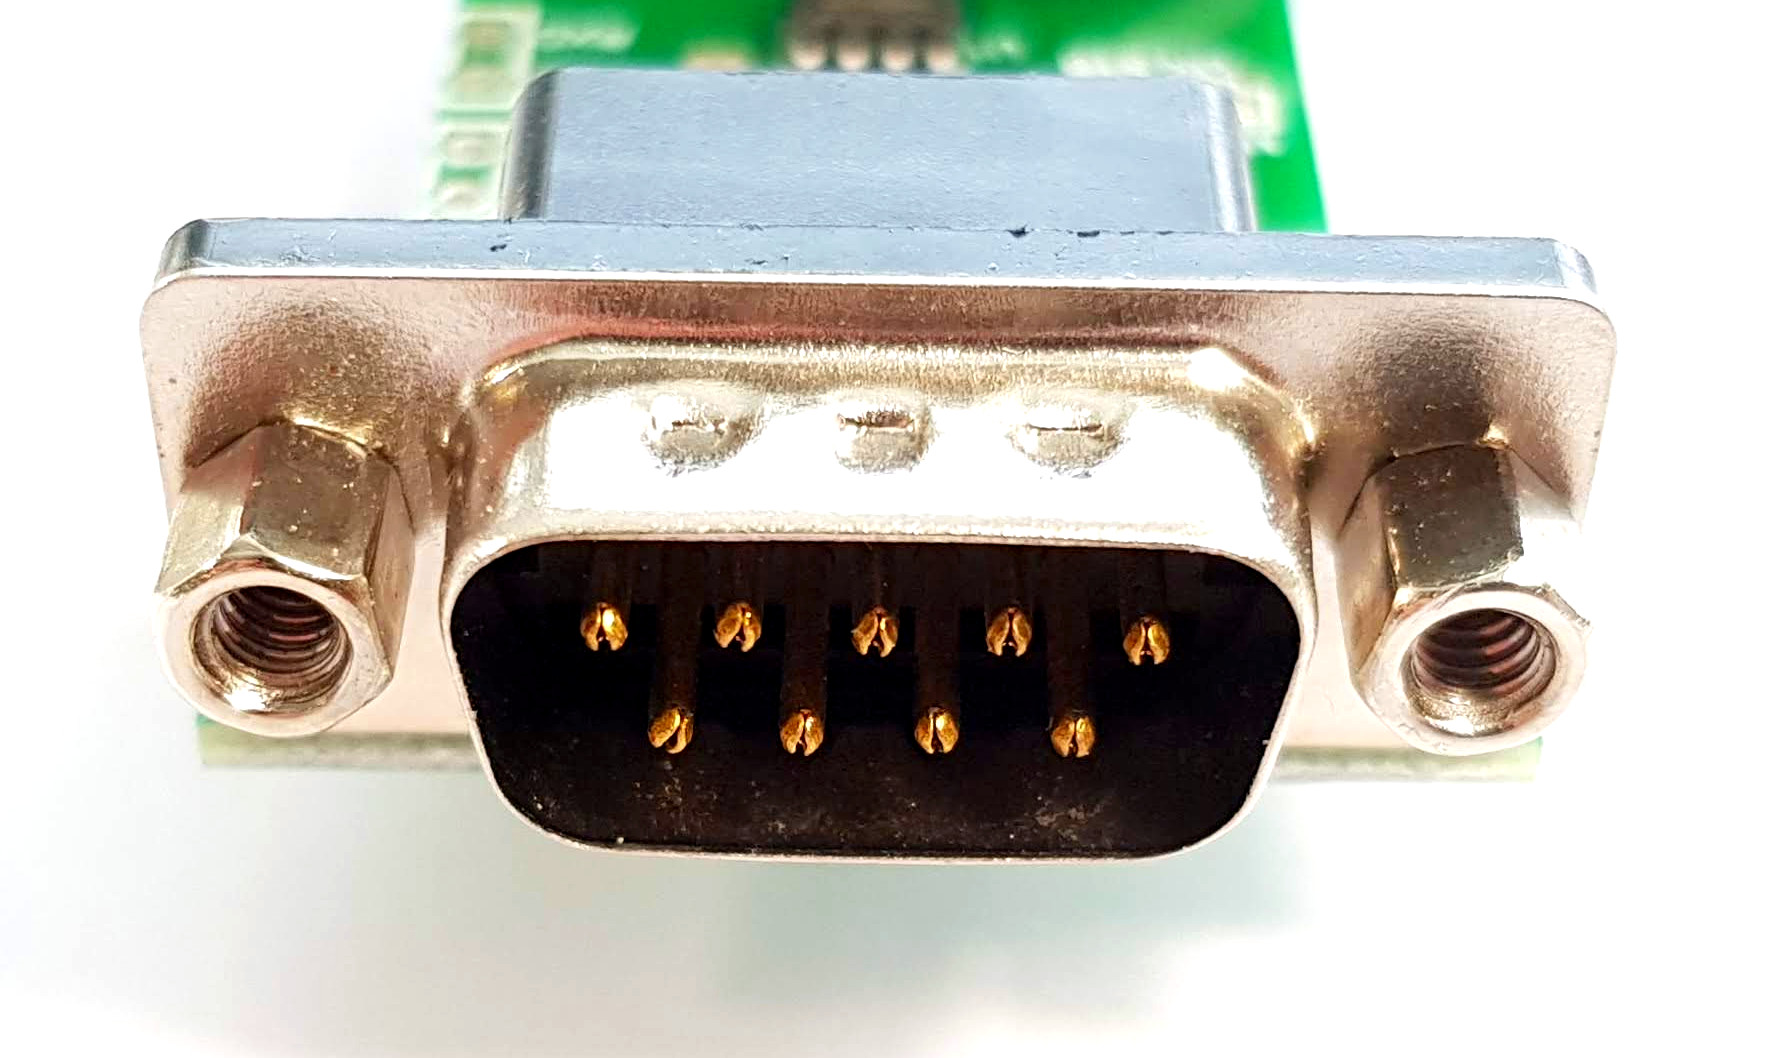
\includegraphics[width=0.45\textwidth]{transport_layer/de-9_connector_male_plug}
    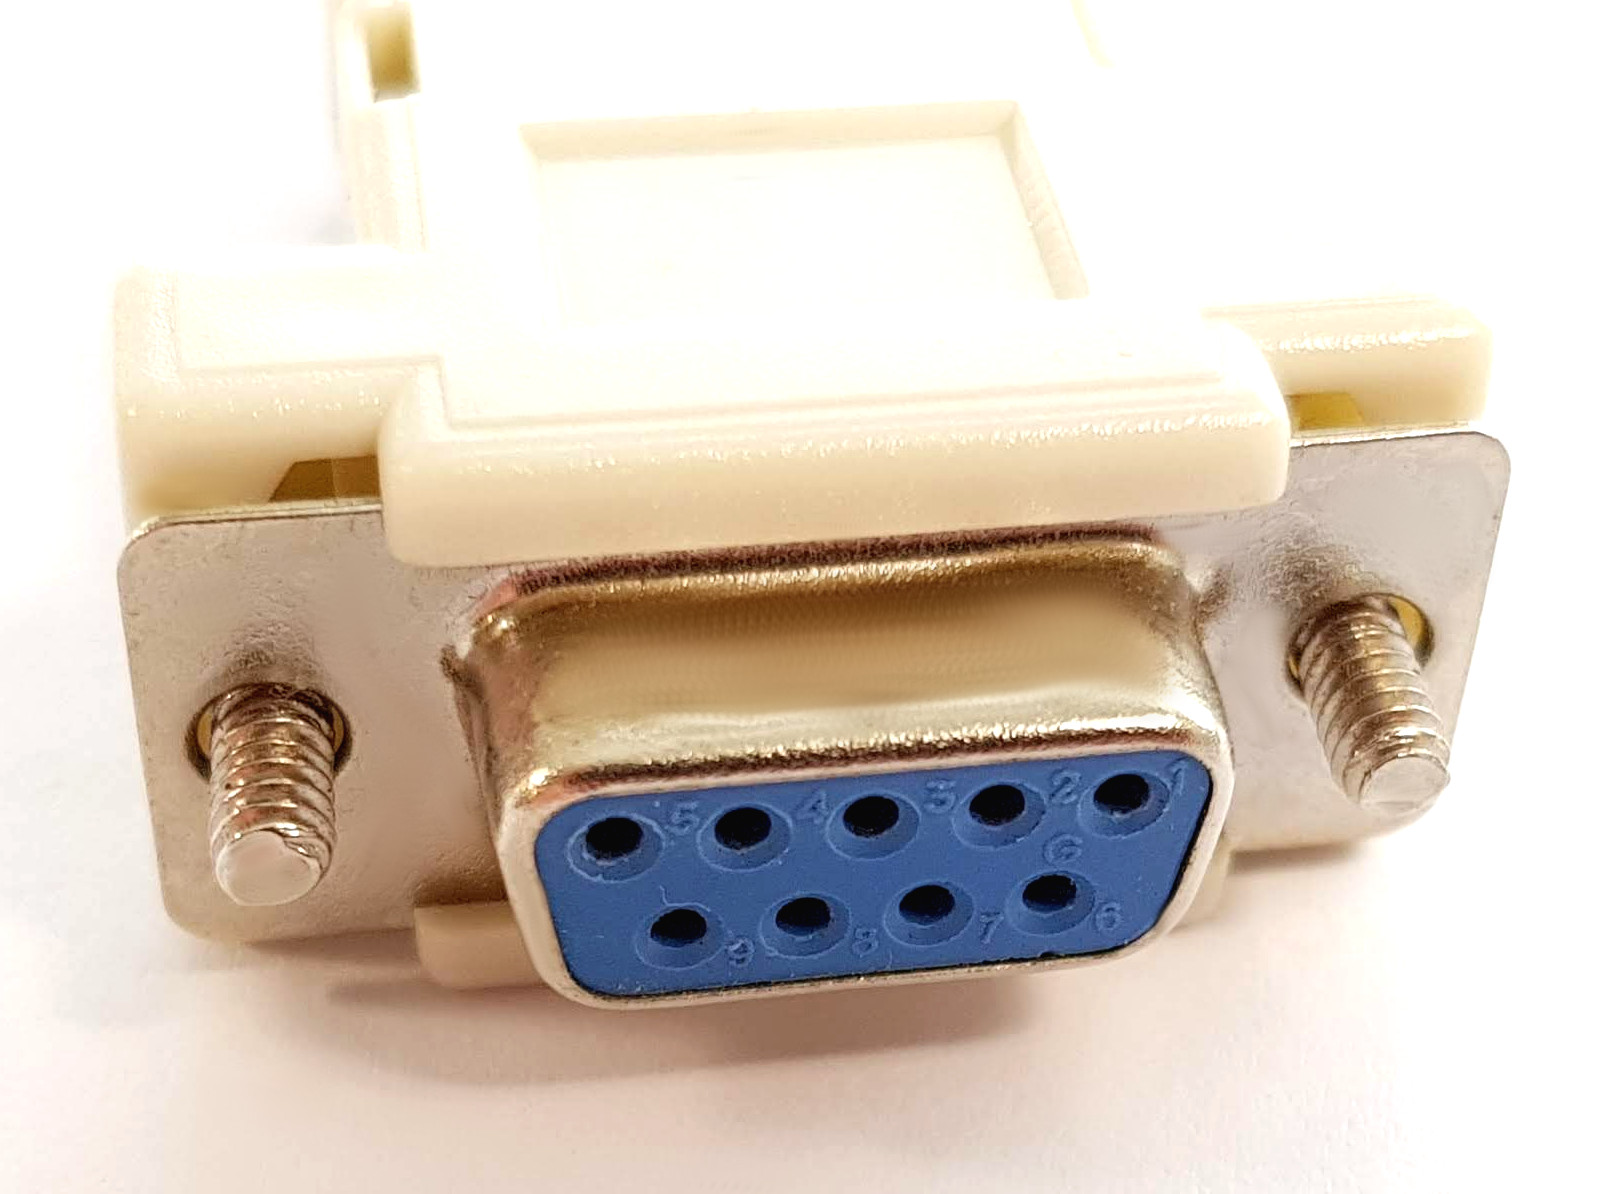
\includegraphics[width=0.45\textwidth]{transport_layer/de-9_cable_female_socket}
    \caption{UAVCAN D-Sub connector pair example: device connector (left) and cable (right).
    \label{fig:can_uavcan_d_sub_connector_example}}
\end{figure}

The UAVCAN D-Sub connector is based on the industry-standard \textbf{D-Sub DE-9} (9-circuit) connector type.
Devices are equipped with the male plug connector type mounted on the panel or on the PCB,
and the cables are equipped with the female socket connectors on both ends
(see the figure \ref{fig:can_uavcan_d_sub_connector_example}).

If the device uses two parallel connectors per CAN bus interface (as recommended),
then all of the lines of the paired connectors,
including those that are not used by the current specification,
must be interconnected one to one.
This will ensure compatibility with future revisions of the specification that make use of
currently unused circuits of the connector.

The CAN physical layer standard that can be used with this connector type is
ISO 11898-2\footnote{Also known as \emph{high-speed CAN}.}.

Devices that deliver power to the bus are required to provide 23.0--30.0 V on the bus power line, 24 V nominal.
The maximum current draw is up to 3 A per connector.

Devices that are powered from the bus should expect 18.0--30.0 V on the bus power line.
The maximum recommended current draw from the bus is 0.5 A per device.

The table \ref{table:can_uavcan_d_sub_pinout} documents the pinout specification for the
UAVCAN D-Sub connector type.
The provided pinout, as has been indicated above, is the de-facto industry standard for the CAN bus.
Note that the signals "CAN High" and "CAN Low" must belong to the same twisted pair.
Usage of twisted or flat wires for all other signals remains at the discretion of the implementer.

\begin{UAVCANSimpleTable}{UAVCAN D-Sub connector pinout}{|l l X|}\label{table:can_uavcan_d_sub_pinout}
    \# & Function           & Note \\
    1  &                    &  \\
    2  & CAN low            & Twisted with "CAN high" (pin 7). \\
    3  & CAN ground         & Must be interconnected with "Ground" (pin 6) within the device. \\
    4  &                    &  \\
    5  & CAN shield         & Optional. \\
    6  & Ground             & Must be interconnected with "CAN ground" (pin 3) within the device. \\
    7  & CAN high           & Twisted with "CAN low" (pin 2). \\
    8  &                    &  \\
    9  & Bus power supply   & 24 V nominal. See the power supply requirements. \\
\end{UAVCANSimpleTable}

\subsubsection{UAVCAN M8 connector}

The UAVCAN M8 connector type is based on the standard circular M8 B-coded 5-circuit connector type,
shown on the figure \ref{fig:can_uavcan_m8_connector_example}.
This is a popular industry-standard connector, and there are many vendors that manufacture compatible components:
connectors, cables, termination plugs, T-connectors, and so on.
The pinning, physical layer, and supply voltages used in this connector type are compatible with CiA 103 (CANopen)
and some other CAN bus standards.

The M8 connector is preferred for most UAVCAN applications (it should be the default choice,
except when there are specific reasons to select another standard connector type).

{
\NoLeftSkip
\begin{UAVCANCompactTable}{X X}
    Advantages & Disadvantages \\
    \begin{itemize}
        \item Compatibility with existing COTS hardware.
        Connectors, cables, termination plugs, and other components can be purchased from many different vendors.
        \item High-reliability options are available from multiple vendors.
        \item Low-cost options are available from multiple vendors.
        \item Reasonably compact. M8 connectors are much smaller than D-Sub.
        \item PCB mounted and panel mounted types are available.
    \end{itemize}
    &
    \begin{itemize}
        \item M8 connectors may be a poor fit for applications that have severe weight and space constraints.
        \item The level of adoption in the industry is noticeably lower than that of the D-Sub connector type.
    \end{itemize}
\end{UAVCANCompactTable}
}

\begin{figure}[hbt]
    \centering
    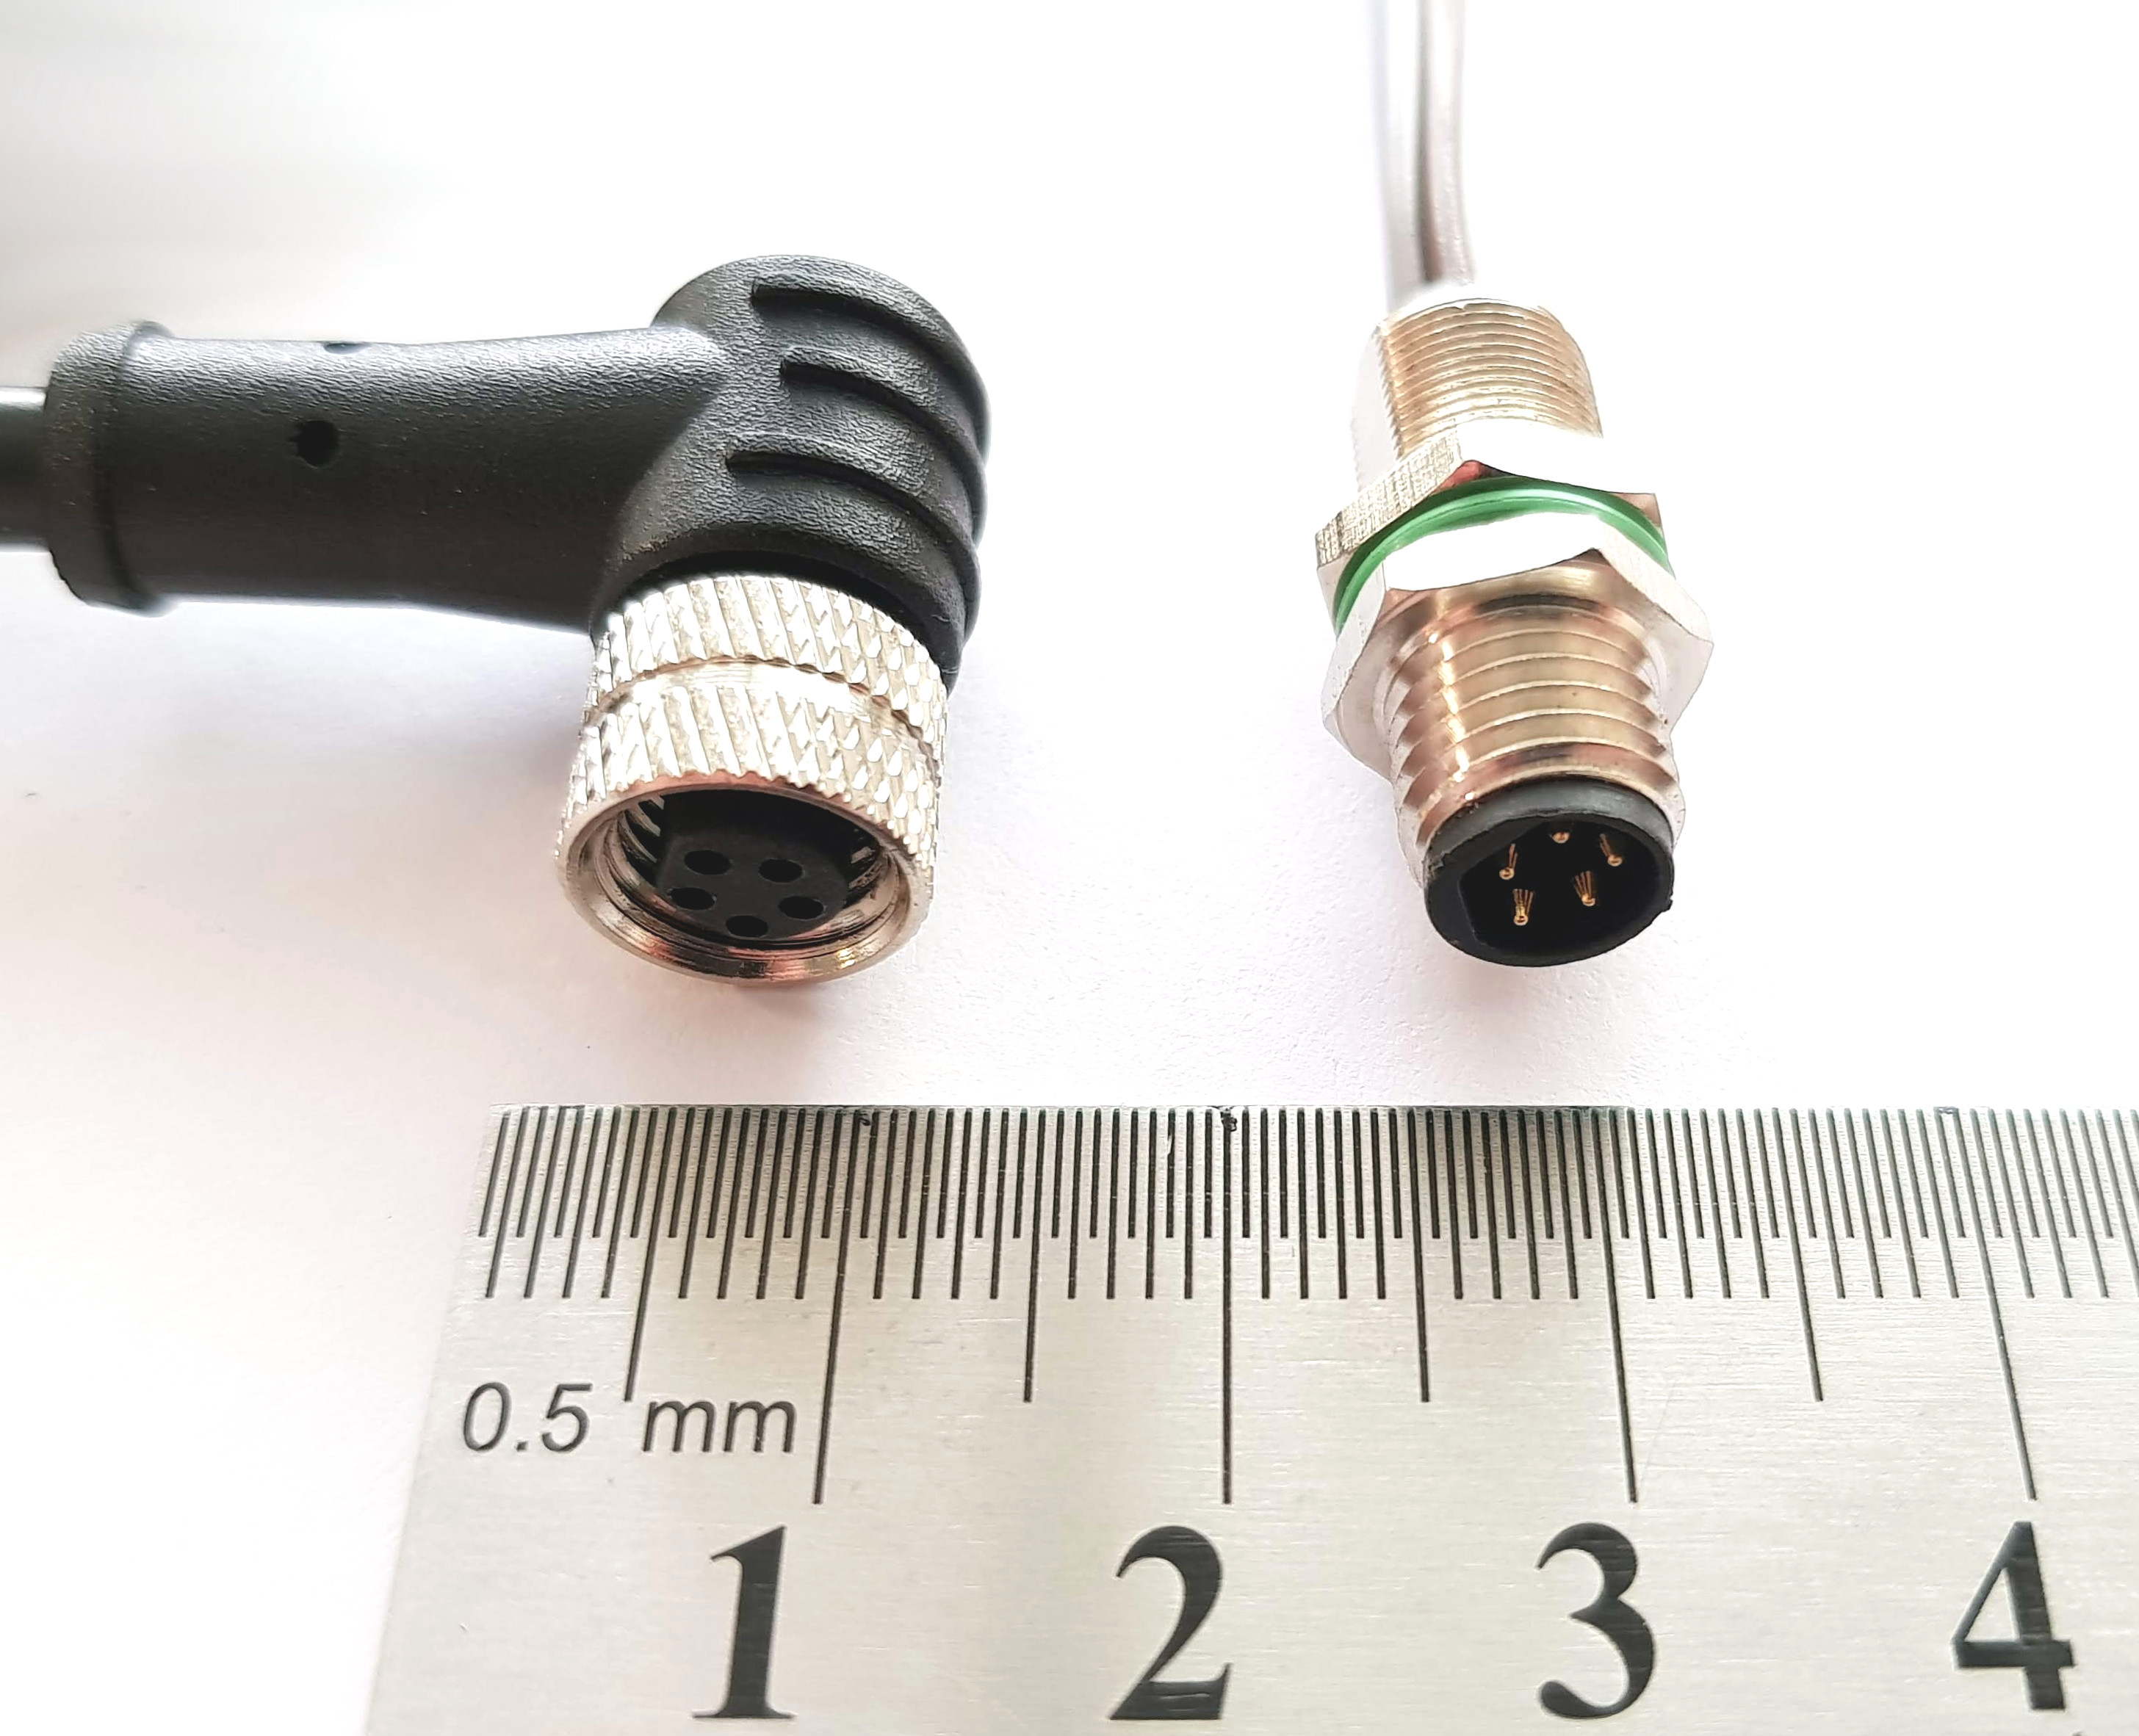
\includegraphics[width=0.7\textwidth]{transport_layer/m8_connector_pair_female_socket_male_plug}\\
    Example connectors: female socket cable (left) and male plug device connector (right).
    Different connector types are available from various vendors: PCB mounted, panel mounted;
    straight cables, angled cables, etc.
    \caption{UAVCAN M8 connector pair example.
    \label{fig:can_uavcan_m8_connector_example}}
\end{figure}

\begin{figure}[hbt]
    \centering
    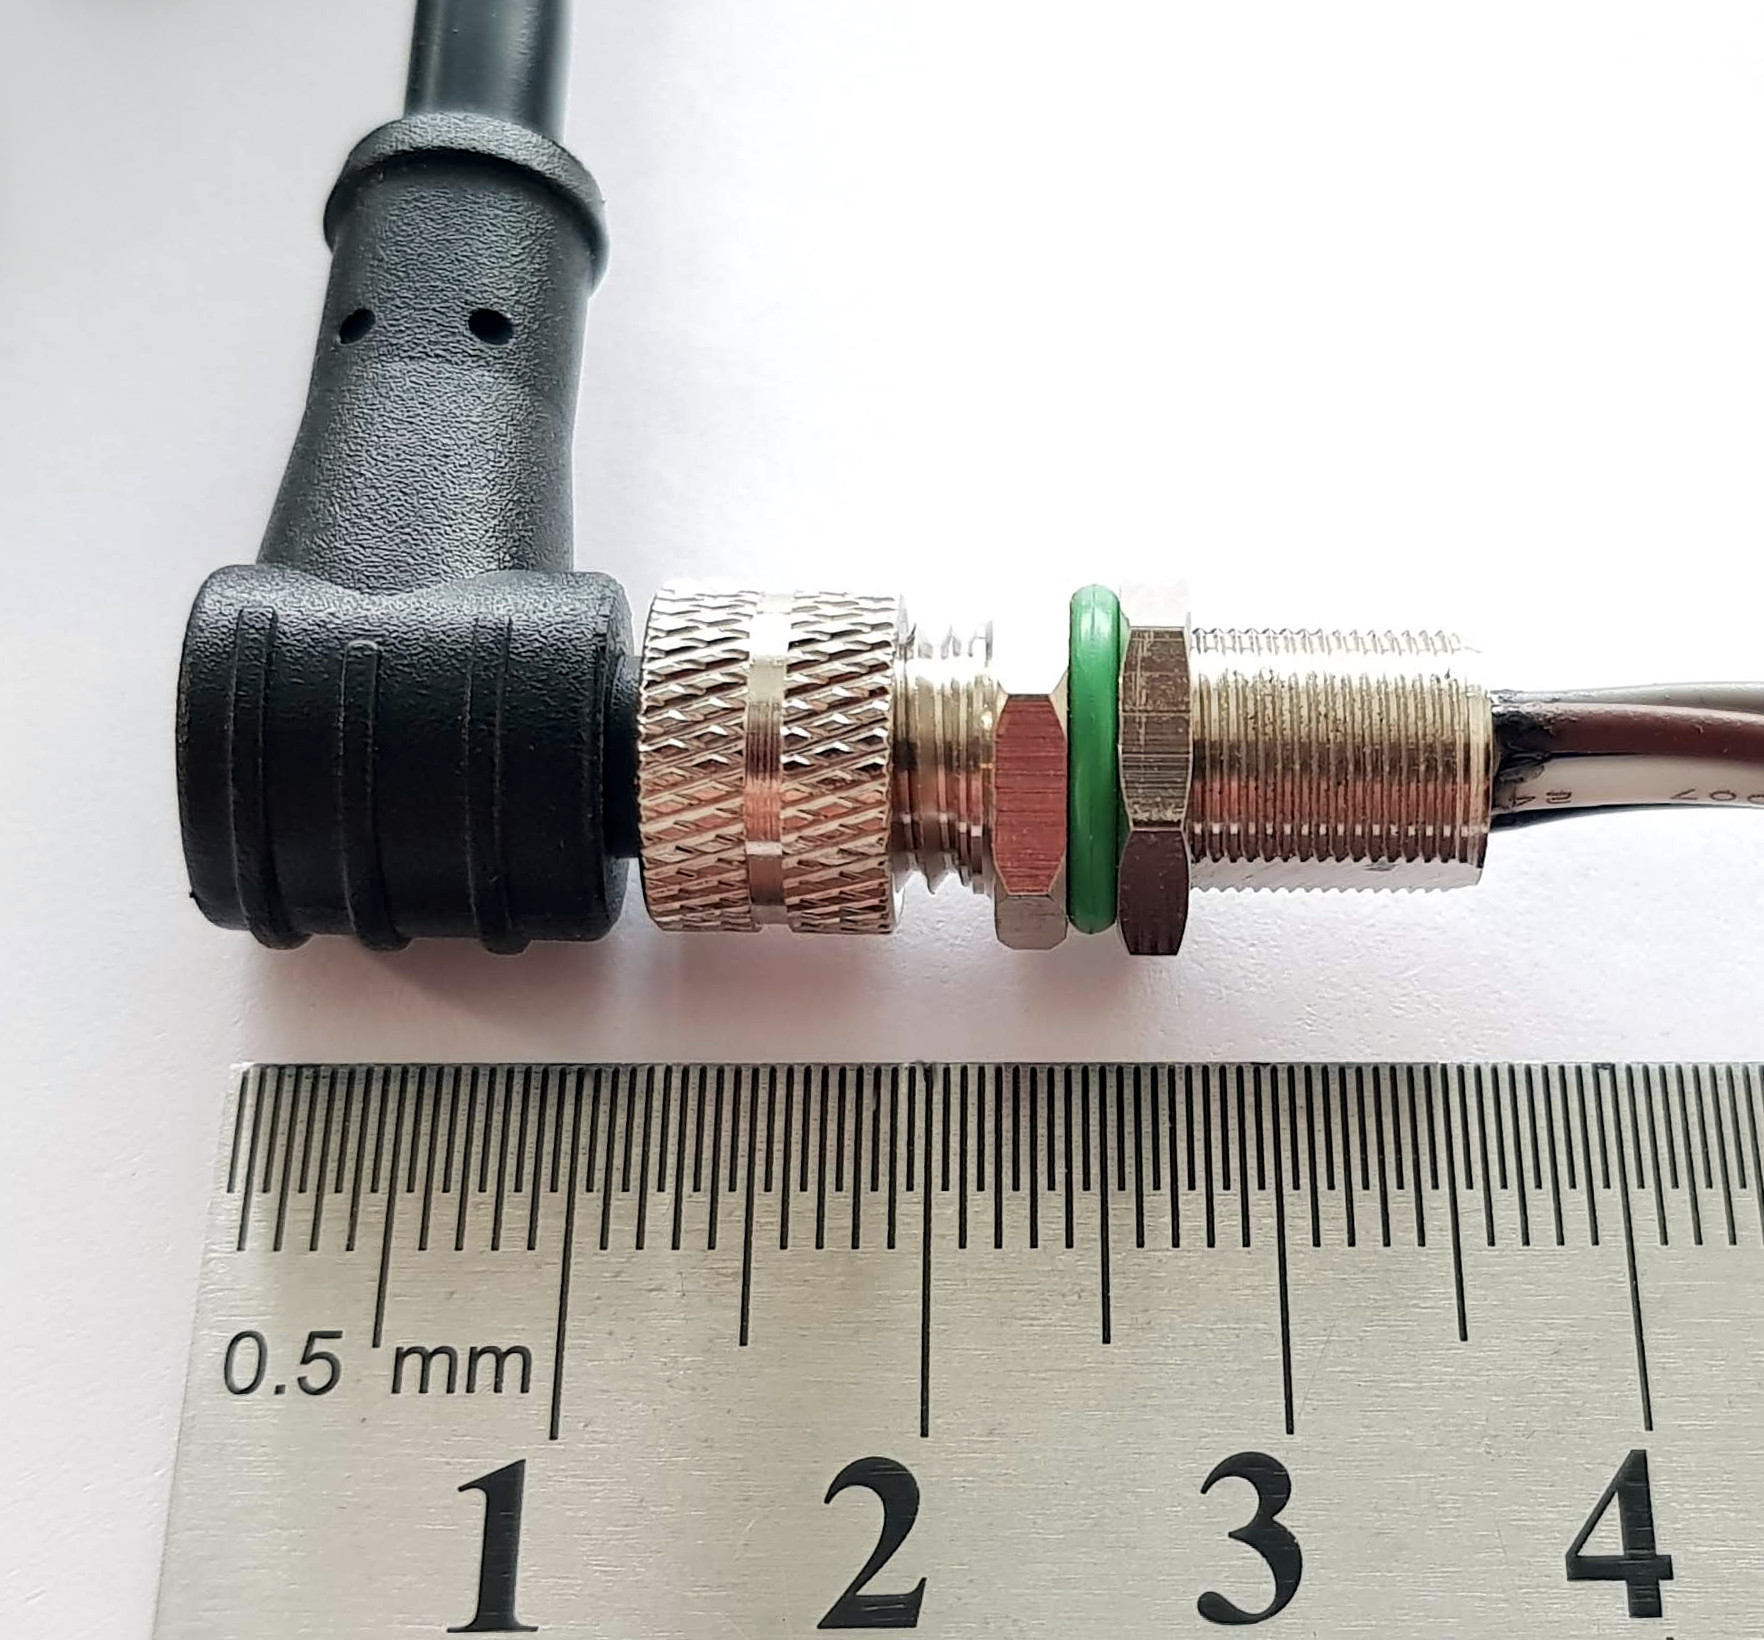
\includegraphics[width=0.7\textwidth]{transport_layer/m8_connector_pair_assembled}
    \caption{UAVCAN M8 assembled connector pair example.}
\end{figure}

The UAVCAN M8 connector is based on the industry-standard \textbf{circular M8 B-coded 5-circuit} connector type.
Devices are equipped with the male plug connector type
mounted on the panel or on the PCB, and the cables are equipped with the female socket connectors on both ends
(see the figure \ref{fig:can_uavcan_m8_connector_example}).
\emph{Do not confuse A-coded and B-coded M8 connectors -- they are not mutually compatible}.

The CAN physical layer standard that can be used with this connector type is
ISO 11898-2\footnote{Also known as \emph{high-speed CAN}.}.

Devices that deliver power to the bus are required to provide 23.0--30.0 V on the bus power line, 24 V nominal.
The maximum current draw is up to 3 A per connector.

Devices that are powered from the bus should expect 18.0--30.0 V on the bus power line.
The maximum recommended current draw from the bus is 0.5 A per device.

The table \ref{table:can_uavcan_m8_pinout} documents the pinout specification for the UAVCAN M8 connector type.
The provided pinout, as indicated above, is compatible with the CiA 103 specification (CANopen).
Note that the wires "CAN high" and "CAN low" should be a twisted pair.

\begin{UAVCANSimpleTable}{UAVCAN M8 connector pinout}{|l l X|}\label{table:can_uavcan_m8_pinout}
    \# & Function           & Note \\
    1  & Bus power supply   & 24 V nominal. See the power supply requirements. \\
    2  & CAN shield         & Optional. \\
    3  & CAN high           & Twisted with "CAN low" (pin 4). \\
    4  & CAN low            & Twisted with "CAN high" (pin 3). \\
    5  & Ground             & \\
\end{UAVCANSimpleTable}

\subsubsection{UAVCAN Micro connector}

The UAVCAN Micro connector is intended for weight- and space-sensitive applications.
It is a board-level connector, meaning that it can be installed on the PCB rather than on the panel.
An example is shown on the figure \ref{fig:can_uavcan_micro_connector_example}.

The Micro connector is compatible with the Dronecode Autopilot Connector Standard.
This connector type is recommended for small UAV and nanosatellites.
It is also the recommended connector for attaching external panel-mounted connectors
(such as the M8 or D-Sub types) to the PCB inside the enclosure.

{
\NoLeftSkip
\begin{UAVCANCompactTable}{X X}
    Advantages & Disadvantages \\
    \begin{itemize}
        \item Extremely compact, low-profile. The PCB footprint is under 9✕5 millimeters.
        \item Secure positive lock ensures that the connection will not self-disconnect when exposed to vibrations.
        \item Low-cost, easy to stock.
    \end{itemize}
    &
    \begin{itemize}
        \item Board-level connections only. No panel-mounted options available.
        \item No shielding available.
        \item Not suitable for safety-critical hardware.
    \end{itemize}
\end{UAVCANCompactTable}
}

\begin{figure}[hbt]
    \centering
    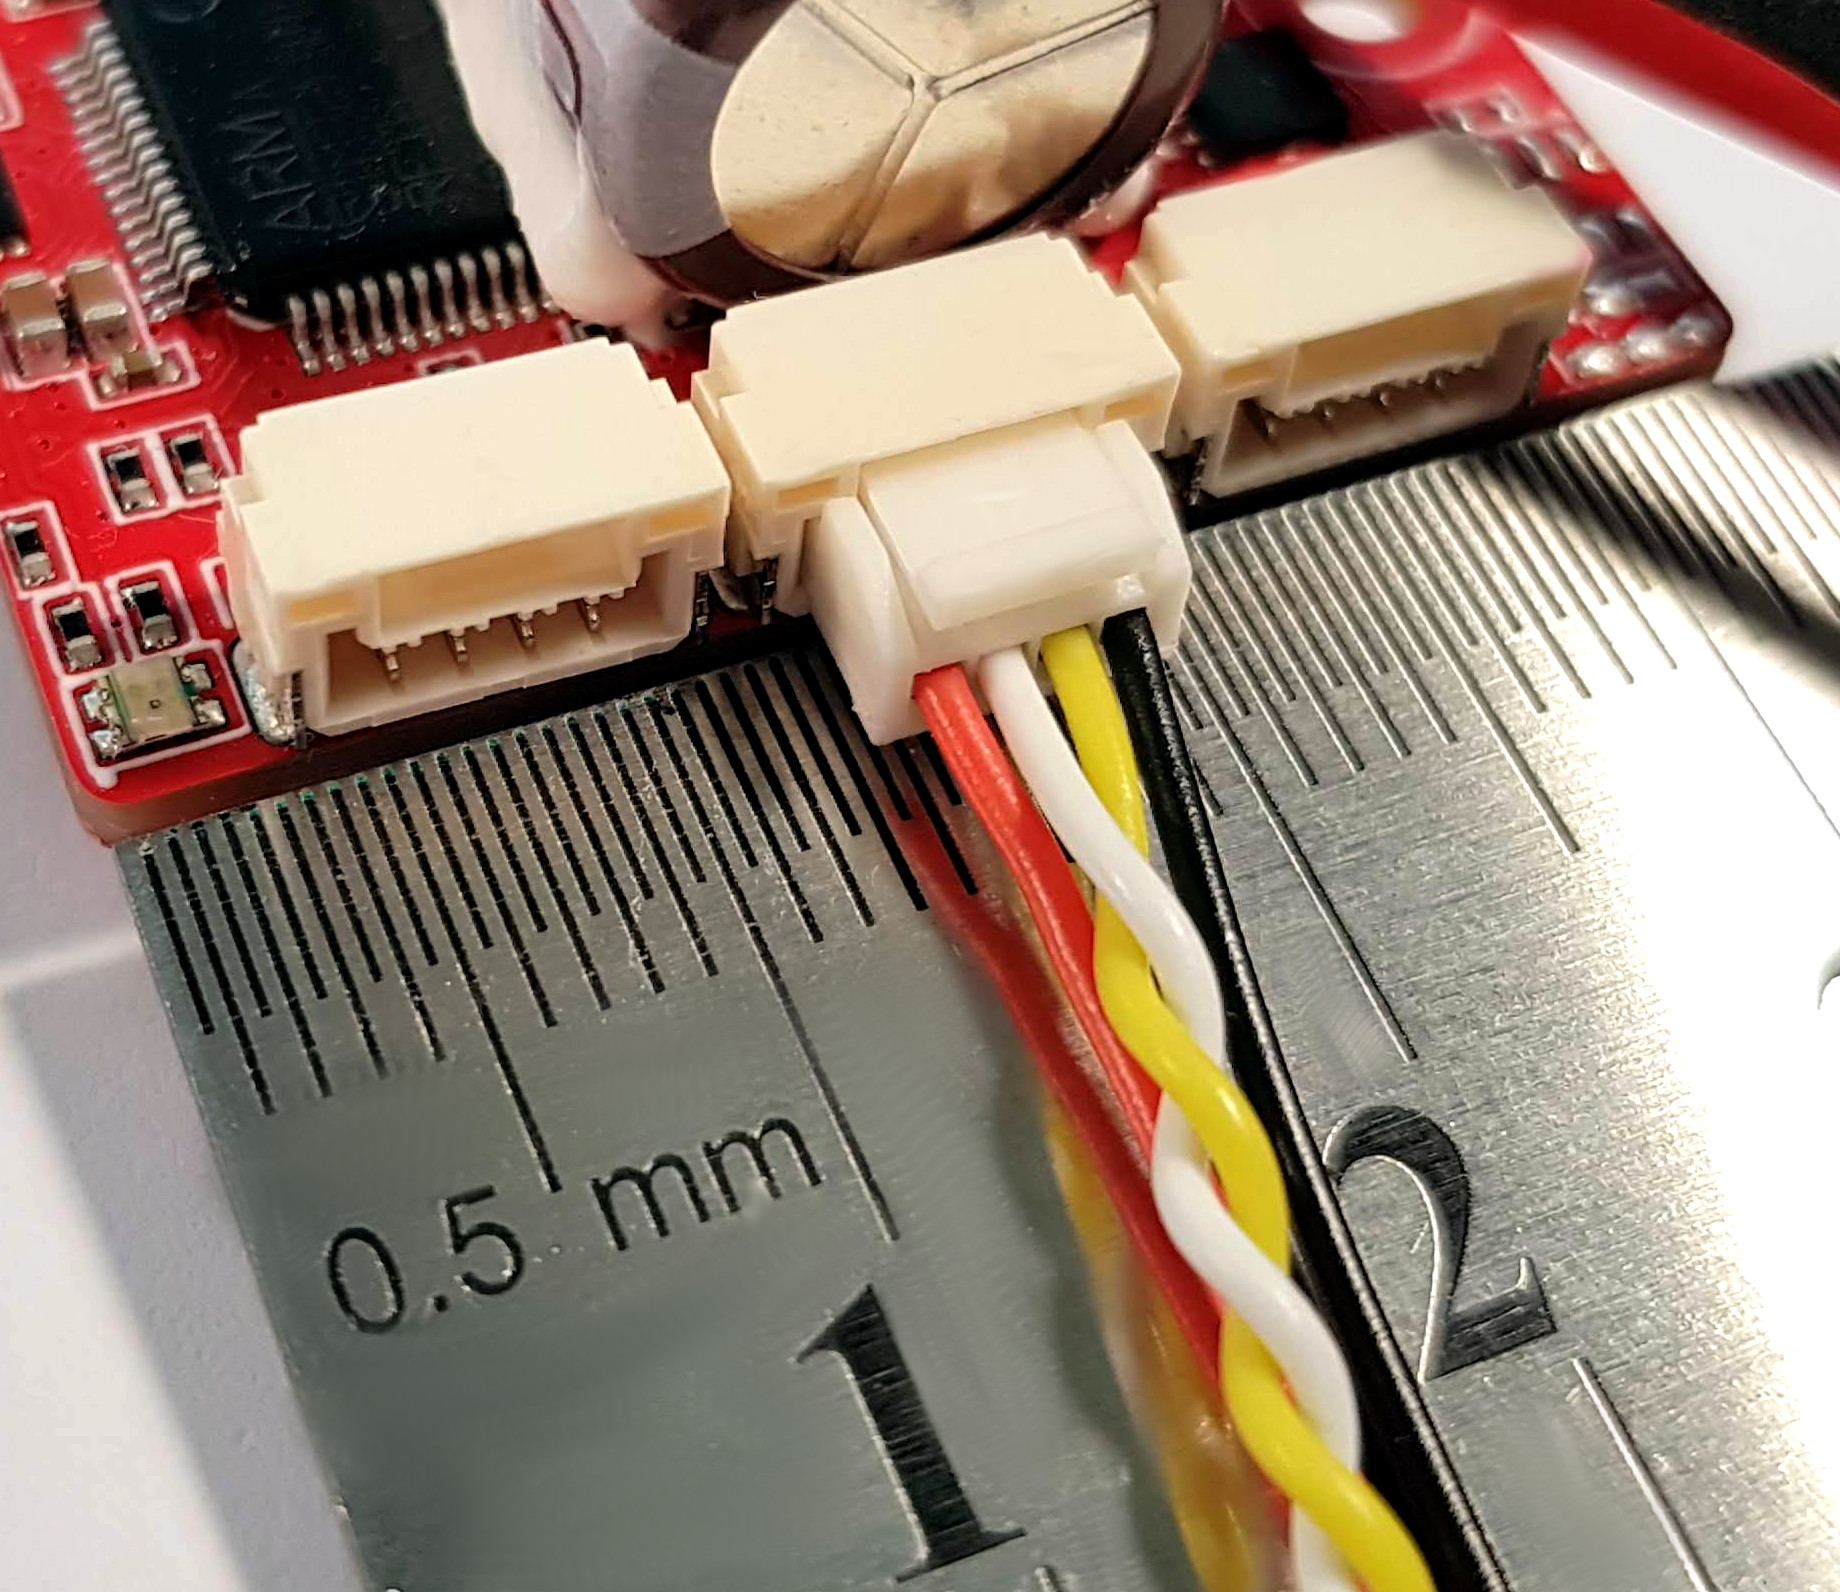
\includegraphics[width=0.7\textwidth]{transport_layer/jst_gh_connectors}
    \caption{UAVCAN Micro right-angle connectors with a twisted pair patch cable connected.
    \label{fig:can_uavcan_micro_connector_example}}
\end{figure}

\begin{figure}[hbt]
    \centering
    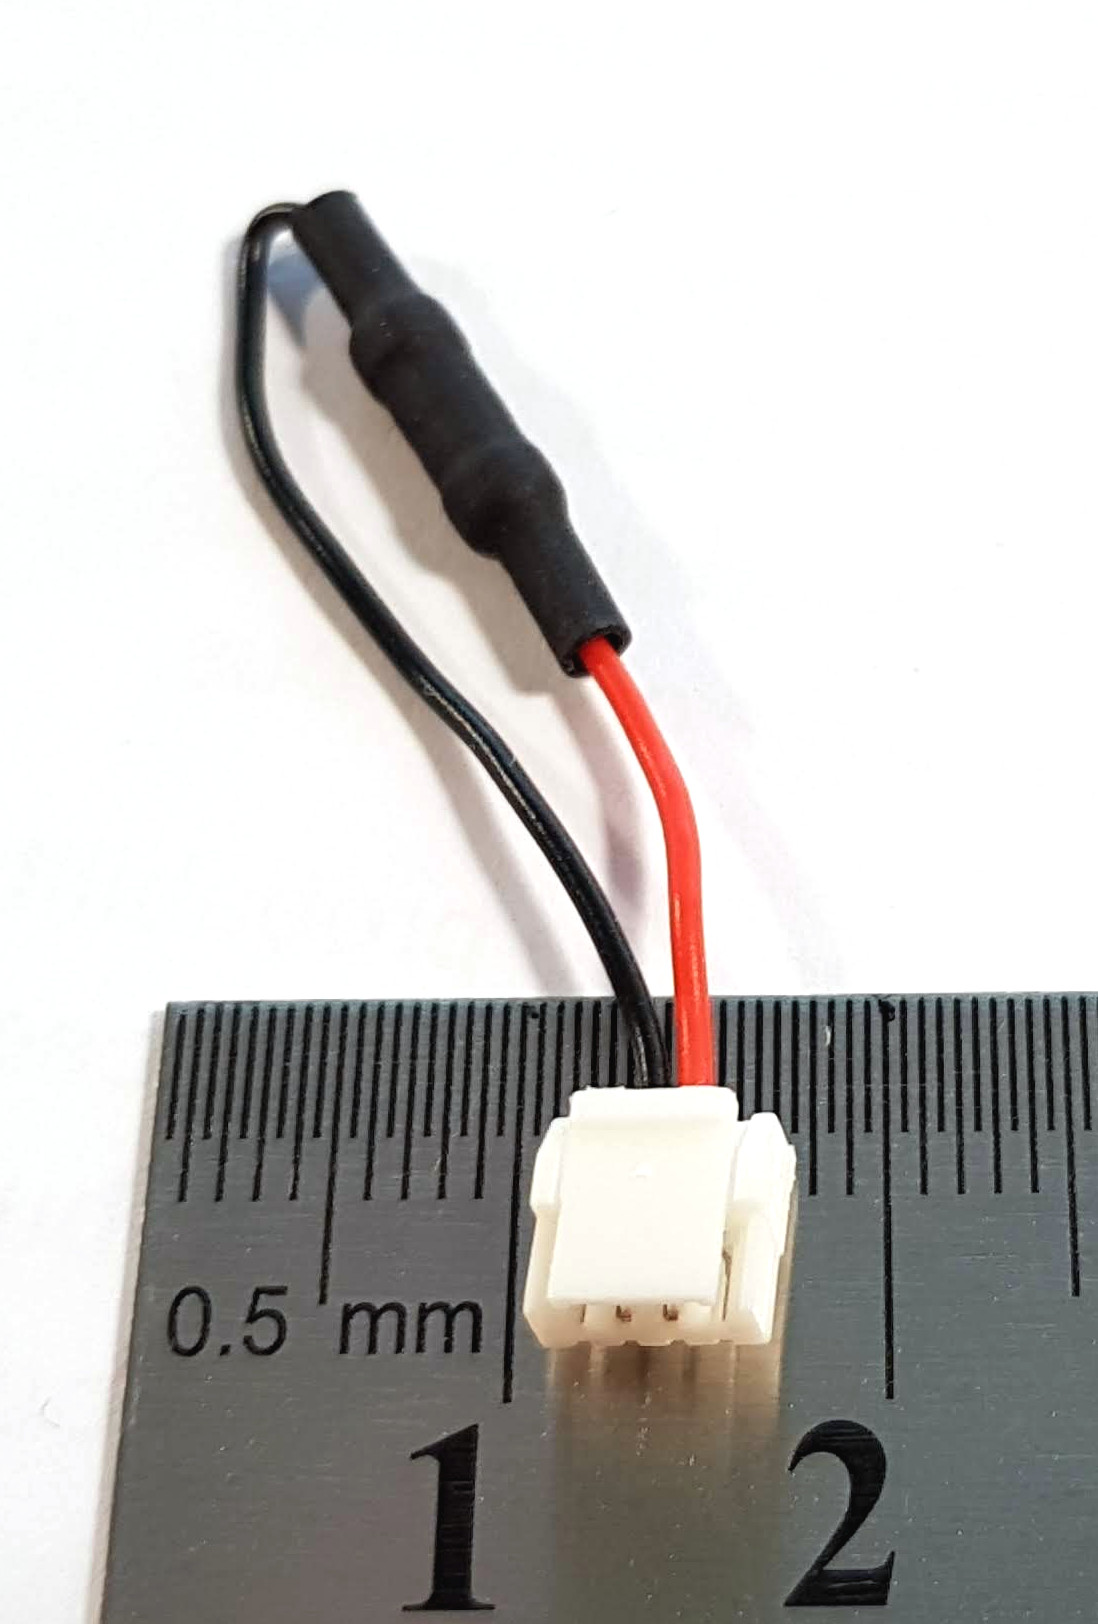
\includegraphics[width=0.3\textwidth]{transport_layer/jst_gh_termination_plug}
    \caption{UAVCAN Micro CAN bus termination plug.}
\end{figure}

The UAVCAN Micro connector is based on the proprietary \textbf{JST GH 4-circuit} connector type.

The suitable cable types are flat or twisted pair \#30 to \#26 AWG,
outer insulation diameter 0.8--1.0 mm, multi-strand.
Non-twisted (flat) cables can only be used in very small deployments free of significant
EMI\footnote{Electromagnetic interference.};
otherwise, reliable functioning of the bus cannot be guaranteed.

The CAN physical layer standard that can be used with this connector type is ISO 11898-2.

Devices that deliver power to the bus are required to provide 5.0--5.5 V on the bus power line.
The anticipated current draw is up to 1 A per connector.

Devices that are powered from the bus should expect 4.0--5.5 V on the bus power line.
The maximum recommended current draw from the bus is 0.5 A per device.

The table \ref{table:can_uavcan_micro_pinout} documents the pinout specification for the UAVCAN M8 connector type.
The provided pinout, as indicated above, is compatible with the Dronecode Autopilot Connector Standard.
Note that the wires "CAN high" and "CAN low" should be a twisted pair.

\begin{UAVCANSimpleTable}{UAVCAN Micro connector pinout}{|l l X|}\label{table:can_uavcan_micro_pinout}
    \# & Function           & Note \\
    1  & Bus power supply   & 5 V nominal. See the power supply requirements. \\
    2  & CAN high           & Should be twisted with "CAN low" (pin 3). \\
    3  & CAN low            & Should be twisted with "CAN high" (pin 2). \\
    4  & Ground             & \\
\end{UAVCANSimpleTable}

\subsection{CAN bus physical layer parameters}

As can be seen from the rest of the specification,
UAVCAN is mostly agnostic of the parameters of the physical layer.
However, vendors should follow the recommendations provided in this section
to maximize the cross-vendor compatibility.

\subsubsection{CAN 2.0}

This section is dedicated to the legacy CAN 2.0 protocol.

The table \ref{table:can_2.0_phy_parameters} lists the standard parameters of the CAN PHY for
ISO 11898-2.
The estimated bus length limits are based on the assumption that the propagation delay does not exceed 5 ns/m,
not including additional delay times of CAN transceivers and other components.

\begin{UAVCANSimpleTable}{UAVCAN Micro connector pinout}{|X[c] X[c] X[c] X[c] X[c]|}
    Bit rate [kbit/s] &
    Valid range for location of sample point [\%] &
    Recommended location of sample point [\%] &
    Maximum bus length [m] &
    Maximum stub length [m] \label{table:can_2.0_phy_parameters} \\

    1000    & 75 to 90  & 87.5  & 40    & 0.3 \\
     500    & 85 to 90  & 87.5  & 100   & 0.3 \\
     250    & 85 to 90  & 87.5  & 250   & 0.3 \\
     125    & 85 to 90  & 87.5  & 500   & 0.3 \\
\end{UAVCANSimpleTable}

Designers are encouraged to implement CAN auto bit rate detection when applicable.
Please refer to the CiA 801 application note for the recommended practices.

UAVCAN allows the use of a simple bit time measuring approach,
as it is guaranteed that any functioning UAVCAN network will always exchange node status messages,
which can be expected to be published at a rate no lower than 1 Hz,
and that contain a suitable alternating bit pattern in the CAN ID field.
Please refer to the chapter \ref{sec:application_layer} for details.

\subsubsection{CAN FD}

This section will be populated in a later revision of the document.
